\subsection{Deep Laplacian Pyramid Network (LapSRN\cite{LapSRN}) and Multi-scale Deep Laplacian Pyramid Network (MS-LapSRN \cite{MSLapSRN})}

\subsubsection{Features}
\textbf{LapSRN} in order to be able to reconstruct the SR image uses:
\begin{itemize}
    \item \textbf{Charbonnier loss} because the L2 loss is not able to capture the underlying mapping of LR images to many HR images.
    \item \textbf{progressive reconstruction} of the SR image using the Laplacian Pyramid 
    Framework \cite{laplacianpyramid}.
    \item \textbf{residual learning}: learn the summation between the laplacian extracted by \textit{features extraction branch} and the upscaled LR image in the \textit{image reconstruction branch}
\end{itemize}
\textbf{MS-LapSRN} improve LapSRN introducing:
\begin{itemize}
    \item \textbf{parameter sharing} across pyramid level and within pyramid levels in order to reduce the amount of parameters which increase with the scale (the greater the scale the deeper the network since there are more levels).
    \item \textbf{local skip connections} for avoiding the vanishing/exploding gradient prolem with the increase in the depth of the network.
    \item \textbf{multi scale training}: the previous network was trained for each scale different networks.
\end{itemize}

\subsubsection{Architecture}
\begin{figure}
    \centering
    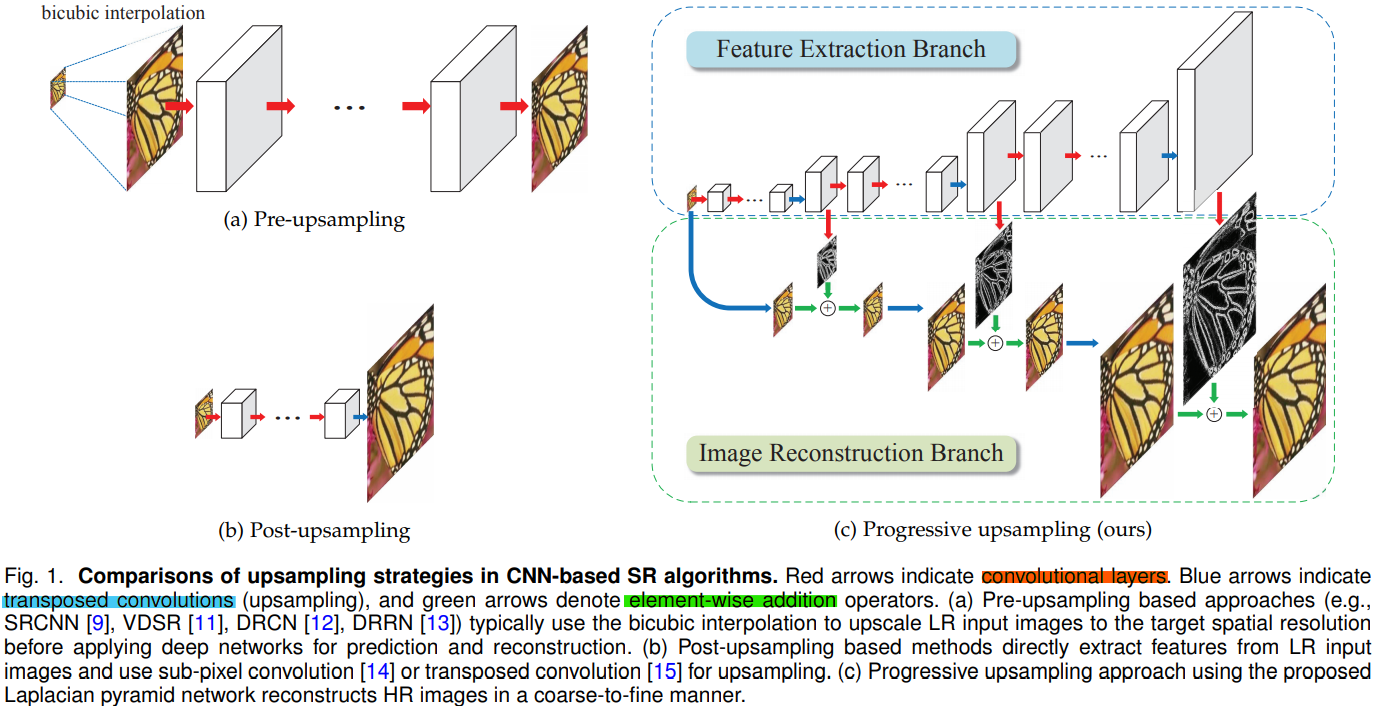
\includegraphics[width=\textwidth, keepaspectratio]{lapsr-old-model.png}
    \caption{LapSRN architecture.}\label{lapsrn:old}
\end{figure}

\begin{figure}
    \centering
    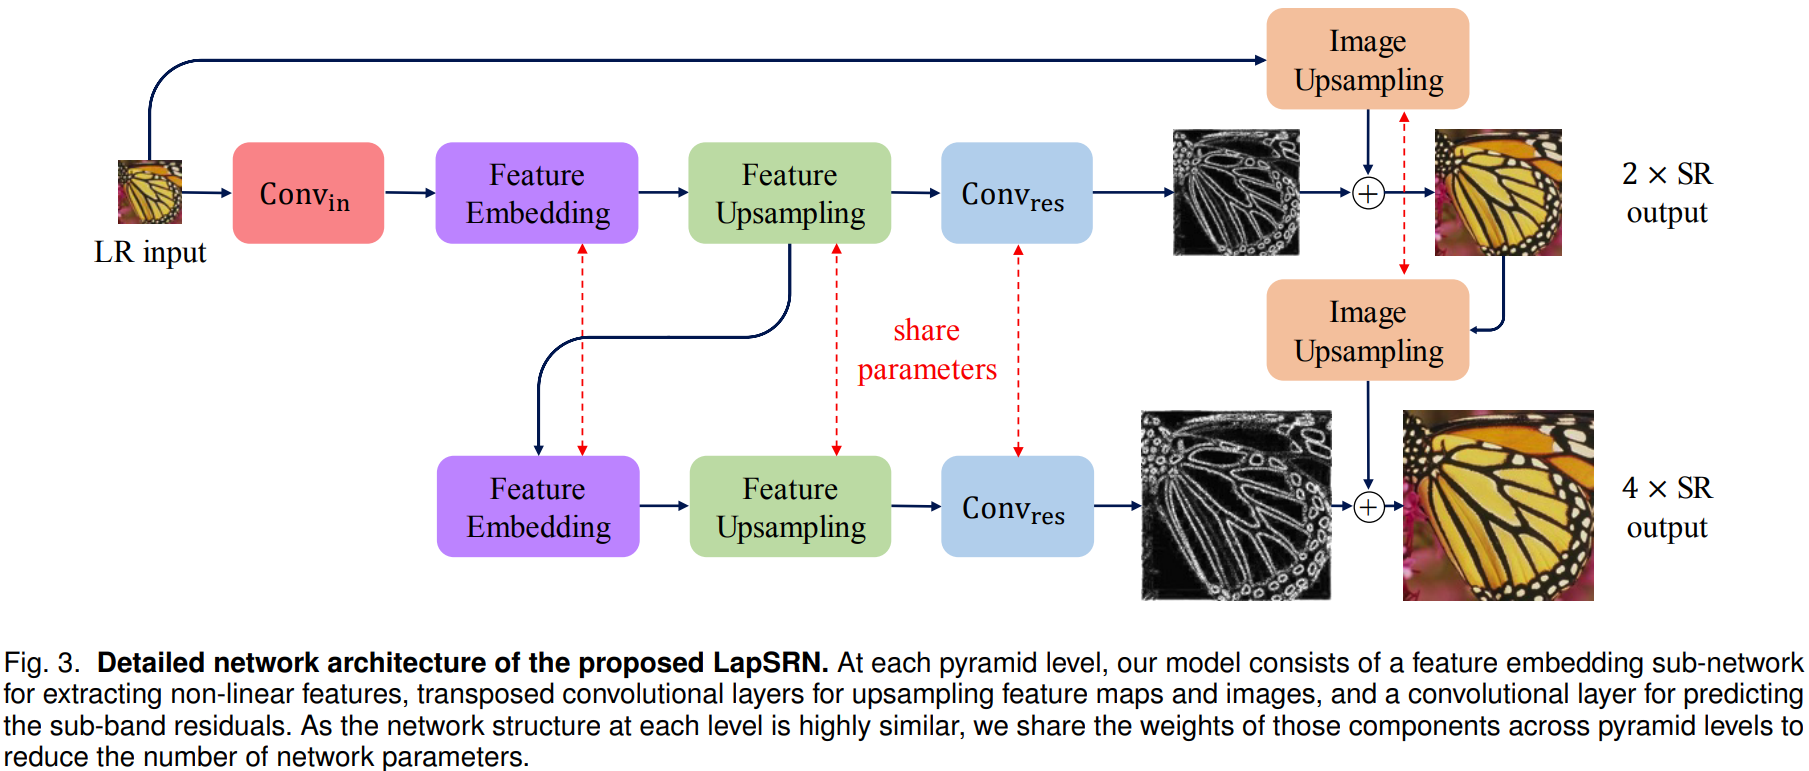
\includegraphics[width=\textwidth, keepaspectratio]{lapsr-new-model.png}
    \caption{MS-LapSRN architecture.}\label{lapsrn:new}
\end{figure}
In \textit{LapSRN} [\Cref{lapsrn:old}] the \textbf{feature extraction branch} extract laplacian representations which are used for training (in an end-to-end fashion) the \textbf{image reconstruction branch} in order to reconstruct the SR image at the last level (due to the laplacian pyramid framework training on an higher scales lead to have also a network capable to resolve SR task for lower scale).

The residual learning allow the network to focus on high-frequency information (edges) instead of low-frequency ones.

In the \textit{MS-LapSRN} [\Cref{lapsrn:new}] the feature extractor ($Conv_{in}$, Feature Embedding, Feature Upsampling, $Conv_{res}$) has always the same function: extract meaningful information from an input image in order to create a residual whose spatial dimension in 2x then the input one; therefore is logic to use same weights for doing so.

The \textit{Feature embedding} has \textbf{R} recursive block \cite{DRCN} \cite{DRRN} which contains distinct \textbf{D} convolutional layers.

\begin{figure}
    \begin{subfigure}{0.49\textwidth}
        \centering
        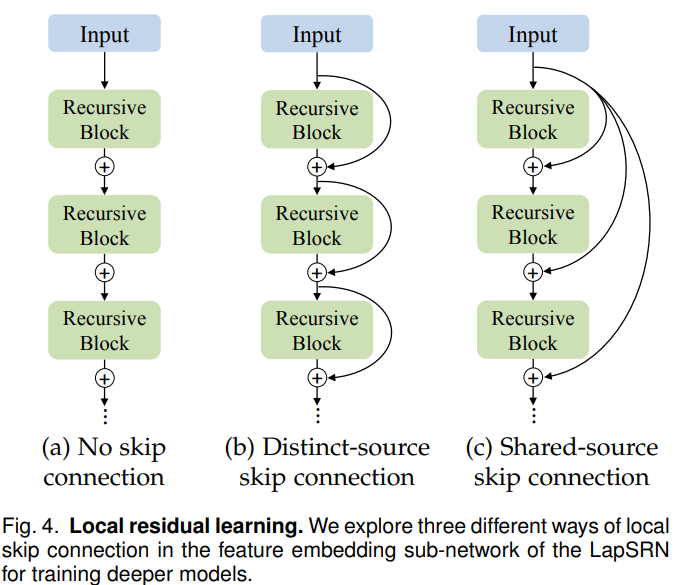
\includegraphics[width=\textwidth, keepaspectratio]{lapsr-recursive-block-differences.png}
        \caption{Differences between local skip connections.}            
    \end{subfigure}
    \begin{subfigure}{0.49\textwidth}
        \centering
        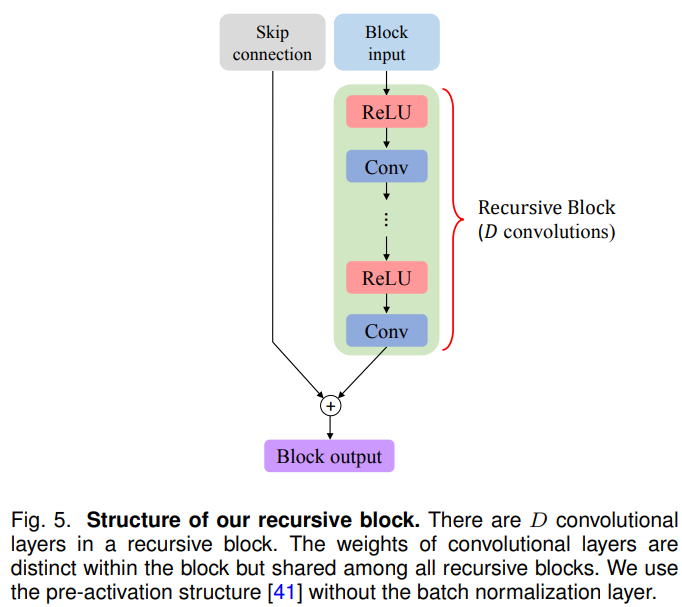
\includegraphics[width=\textwidth, keepaspectratio]{lapsr-recursive-block.png}
        \caption{Recursive block used in MS-LapSRN.} \label{lapsrn:recursiveblock}
    \end{subfigure}
\end{figure}

The structure of the recursive block [\Cref{lapsrn:recursiveblock}] use a skip connection directly connected to the input and a pre-activation inside the residual path \cite{resnetidentity}.

\subsubsection{Loss}
Each level s has its own loss function and target ground truth.

The \textbf{Charbonnier loss} function is :
$$
L_S = \frac{1}{N} \sum_{i=1}^{N}\sum_{l=1}^{L} \rho \times \left( \left( y_l^{(i)}-x_l^{(i)} \right) - r_l^{(i)} \right)
$$
where $S$ is the target upsampling factor, $\rho = \sqrt{x^2+\epsilon^2}$ (Charbonnier penalty function which is a differentiable L1 norm), $x_l$ is the upscaled LR image at level l, $y_l$ is the downscaled HR target image (y) at level l and $r_l$ is the residual at level l. 

The final loss is the sum of the loss for each level trained using images with different scales (\textbf{multi scales training}).

\subsubsection{Results}

Here will be presented only the results of \textbf{MS-LapSRN}\cite{MSLapSRN} since it's an evolution of LapSRN.

%TODO
